\section{Vehicle Routing Problem}
\label{sec_vrp_intro}

In the traveling salesman problem (TSP), we find the shortest route that visits each node in a graph exactly once and returns to the starting node. TSP is one of the most widely studied problems in combinatorial optimization both due to its NP-hard nature and as well as its wide variety of practical applications. The vehicle routing problem (VRP) is a generalization of TSP where one or more vehicles are expected to visit the nodes in a graph, usually to satisfy customer demand. VRP is also a well studied topic and has very important applications, especially in supply chain and logistics. These real-life applications lead to many variants of VRP with different constraints, such as  capacitated vehicles, pickups and deliveries on the route, time windows associated with each pickup and delivery etc. 

An important extension of VRP is where some of the information about the graph is revealed over time, such as demand at each node and travel time. This class of VRP is called dynamic VRP (DVRP, also known as real-time or online VRP). Stochastic VRP (SVRP) is where one or more problem parameters are stochastic with some known probability distributions (as opposed to arbitrary or adversarial distributions). In many real-life applications, the relevant VRP is both stochastic and dynamic (SDVRP), which is also focus of this work. We formulate a variant of SVRP and compare solution approaches from the Operations Research (OR) and Reinforcement Learning (RL) literature.

\subsection{Problem Formulation}
\label{sec_vrp_pf}

We consider a decentralized version of the VRP. Consider a delivery driver using a phone app, orders arrive on the app in a dynamic manner. Each order has a delivery charge known to the driver at the time of order creation, and it is assigned to a location in the city. "City" here means the whole Euclidean space in which the VRP problem lives. The city consists of mutually exclusive zones ($num\_zones = 4$) that generate orders at different rates ($order\_probs\_per\_zone = (0.5, 0.3, 0.1, 0.1)$) and with rewards according to truncated normal distribution with different ranges ($order\_reward\_max = (12, 8, 5, 3), order\_reward\_min = (8, 5, 2, 1)$). The orders have a delivery time limit ($order\_promise = 60$), the timer starts with the order creation and is same for all orders. The driver has to accept an order and pick up the package from a given location prior to delivery. Orders that are not accepted disappear probabilistically ($order\_timeout\_prob = 0.15$) when other drivers accept the orders. The vehicle has a capacity limit ($driver\_capacity = 4$), but the driver can accept unlimited orders and plan their route accordingly.  
%there is no limit on the number of orders that are accepted (but not picked up or delivered) by the driver at the same time. Finally, 
Each time step and unit distance travelled adds a fixed cost $(penalty\_per\_timestep = 0.1, \ penalty\_per\_move = 0.1)$, and the episode length is $1000$. The driver's goal is to maximize the total net reward. Our formulation is known as stochastic and dynamic capacitated vehicle routing problem with pickup and delivery, time windows and service guarantee. % (SDPDPTW with service guarantee).

\subsection{Related Work} \label{sec_vrp_related_work}
There is a substantial literature on VRP~\cite{EKSIOGLU20091472}. The closest VRP variant to the problem considered in this paper is the Pickup and Delivery Problem with Time Windows (PDPTW) \cite{Cordeau2008}, which has some additional complexities over vanilla VRP. Due to such complexities, there are fewer exact solution approaches \cite{LuDessouky2004,MAHMOUDI201619}, and a majority of the literature focuses on heuristics. When the problem is also stochastic and dynamic, exact solution methods become intractable except for very specific problem settings. In such cases, anticipatory algorithms that simulate sample future scenarios and merge solutions to those samples are a common choice \cite{BERBEGLIA20108, Berhan2014, Ulrike2016, Ghiani2012}.

Reinforcement Learning (RL) methods have been successfully used for solving the Traveling Salesman Probelm (TSP). \citet{bello2016neural} employ a pointer network \cite{vinyals2015pointer} to optimize the policy, and train an actor-critic algorithm with the negative tour length as the reward signal. \citet{khalil2017learning} develop a single model based on graph embeddings. They use the DQN algorithm to train a greedy policy and graph embedding network simultaneously.  For VRP, \citet{kool2018attention} utilize the Transformer architecture \cite{vaswani2017attention} to develop a model fully based on attention layers. Their proposed model is trained by policy gradients with a greedy baseline, and evaluated on both standard Capacitated VRP (CVRP) and Split Deliverry VRP (SDVRP). \citet{nazari2018reinforcement} further improve the algorithm using embedded inputs and allow the customers and their demands to be stochastic. Besides, \citet{lin2018efficient} propose a contextual multi-agent reinforcement learning framework for fleet management, and use a simulator that mimics the process of online order generation/asignment in real world.

%While traditional VRP focuses on minimizing the tour length, we extend this criterion to integrate order values to learn if the agent can prioritize profitable orders. We consider a more complex environment with multiple zones with different order distributions. In addition, we have time limits for service guarantee. We believe these changes translate better to practical use cases. We also show that a simple 2-layer neural network suffices to learn good policies even in such complex environments.

\subsection{Baseline Algorithm}
We modify the classical three-index Mixed Integer Programming (MIP) formulation \cite{LuDessouky2004,RopkeCordeau2009, FURTADO2017334}. This deterministic MIP is solved for the available orders in the environment. It is further resolved when a new order arrives, if one of the existing orders expires or, when all of the actions are executed. When we solve the MIP, orders already accepted or in transit are modeled as starting conditions. The details of our MIP model is given in Appendix \ref{appendix:vrp_mip}. We leave anticipatory models to future work (see Section \ref{sec_vrp_related_work}).

%Note that when the MIP is solved, some of the orders could have been accepted due to the previous solution and some of the orders could be already in transit. Our version of the model (as opposed to the classical formulation in literature) enforces such starting conditions. 

\ifx
\subsubsection*{Sets}
\begin{vardefs*}
V & Current vehicle location, $V=\{0\}$ \\
P & Pickup nodes (copies of the restaurant nodes, associated with the orders that are not in transit)  \\
D & Delivery nodes representing the orders that are not in transit, $D = \{j | j= i + n, i \in P, n=|P| \}$  \\
A & Nodes representing the orders that are accepted by the driver; $A \subset D$ \\
T & Delivery nodes representing the orders that are in transit  \\
R & Nodes representing the restaurants, used for final return) \\
N & Set of all nodes in the graph, $N = V \cup P \cup D  \cup T \cup R $\\
E & Set of all edges, $E=\{(i, j),  \forall i, j \in N\}$
\end{vardefs*}


\subsubsection*{Decision variables}
\begin{vardefs*}
 x_{ij} & Binary variable, 1 if the vehicle uses the arc from node $i$ to $j$, 0 otherwise; $i, j \in N$ \\
y_{i}  & Binary variable, 1 if the order $i$ is accepted, 0 otherwise; $i \in P$\\
Q_{i} & Auxiliary variable to track the capacity usage as of node  $i$; $i \in N$ \\ 
B_{i} & Auxiliary variable to track the time as of node  $i$; $i \in N$
\end{vardefs*}

\subsubsection*{Parameters}
\begin{vardefs*}
n & Number of orders available to pick up, $n = |P|$ \\ 
c_{ij} & Symmetric Manhattan distance (in miles) matrix between node $i$ and $j$, $(i, j) \in E$ \\
q_i & Supply (demand) at node $i$, $q_0 = |T|; q_i = 1, \forall i \in P;  q_i = -1, \forall i \in D \cup T; q_i = 0 \in R$  \\ 
l_i & Remaining time to deliver order $i$, $i \in D \cup T$ \\ 
m & Travel cost per mile \\
r_i & Revenue for order associated with pick up node $i$, $i \in P$  \\
U & Vehicle capacity  \\
M & A very big number  \\ 
t & Time to travel one mile  \\
d & A constant positive service time spent on accept, pickup, delivery
\end{vardefs*}

\subsubsection*{Model}
\begin{equation}
\begin{array}{rrclcl}
& \max_{x, y, Q, B} & \multicolumn{3}{l}{ \sum_{i \in P} r_i y_i - m \sum_{(i,j) \in E} c_{ij} x_{ij}  } \\  
& \textrm{s.t.} \qquad  \sum_{j \in N} x_{ij}   &=& y_i & \forall i \in P \\   %leave
& \sum_{j \in N} x_{ij} - \sum_{j \in N} x_{i+n,j}  & = & 0 & \forall i \in P  \\     %pickup
& y_i & =& 1 & \forall i \in A \\  % accepted
& \sum_{j \in N} x_{ij}   &=& 1 & \forall i \in V \cup T \\  % start and  in-transit
& \sum_{i \in N \setminus R } \sum_{j \in R }  x_{ij}   &=& 1  &\\     %end 
& \sum_{j \in N \setminus R } x_{ji} - \sum_{j \in N} x_{ij}  & = & 0 & \forall i \in P \cup D \cup T  \\     %flow
& Q_i + q_j - M (1-x_{ij} ) &\leq& Q_j & \forall i,j \in N \\  %captrack
& \max{(0, q_i)}    &\leq& Q_i & \forall i \in N \\  %cap_lb
& \min{(U, U+q_i)}    &\geq& Q_i & \forall i \in N \\  %cap_ub
& B_i + d + c_{ij} t -  M (1-x_{ij} )  &\leq& B_j   & \forall i,j \in N \\  %time_track , *\mathcal{1}\{ i \notin V  \}
& B_i +  c_{i, i+n} t -  M (1- y_i )  &\leq& B_{i+n}  & \forall i \in P \\ %precedence
&  d \sum_{i \in P \setminus A}  y_i  & = & B_0  \\ %timetoaccept
& B_i  &\leq& l_i  & \forall i \in D \cup T \\ %precedence
& x_{ij}, y_i &\in& \{0, 1\} & \forall i,j \in N  \\ 
\end{array}
\end{equation}
\fi

\begin{figure*}[h!]
	\centering
	\begin{subfigure}[b]{0.45\textwidth}
		\centering
		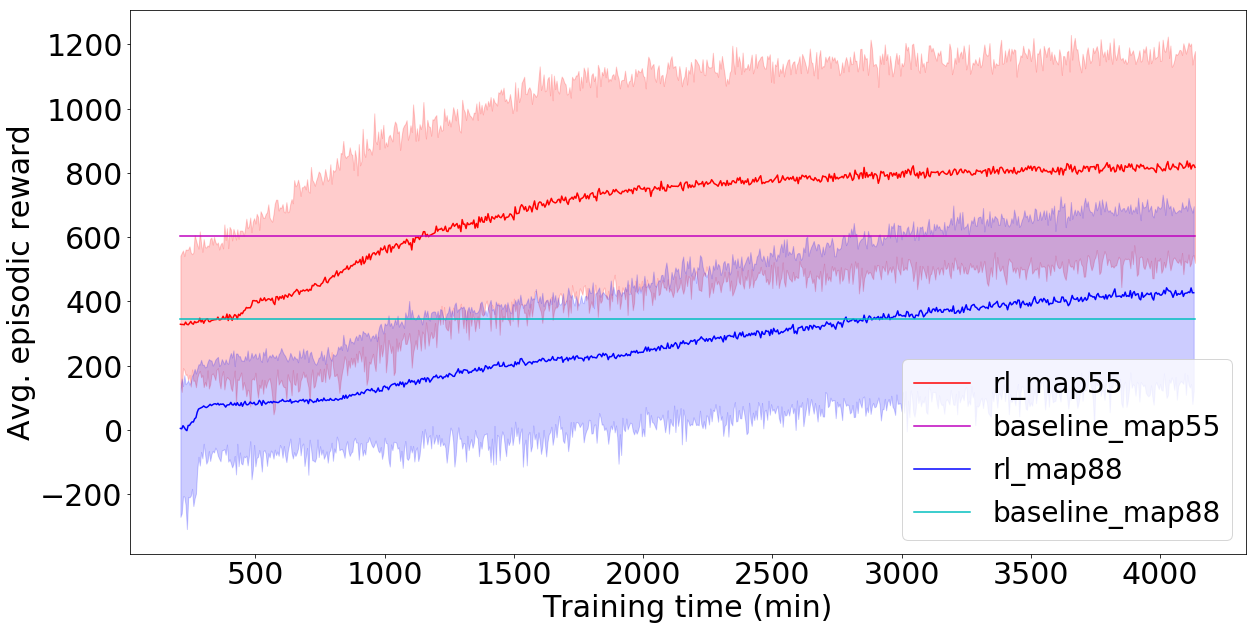
\includegraphics[width=1\linewidth]{vrp_images/vrp_mapsize.png}
		\caption{RL vs baseline solution for VRP with 3 pick-up locations, 5 orders and map sizes $5 \times 5$ and $8 \times 8$ }
		\label{fig:vrp_mapsize}
	\end{subfigure}
	\hspace{2em}
	\begin{subfigure}[b]{0.45\textwidth}
		\centering
		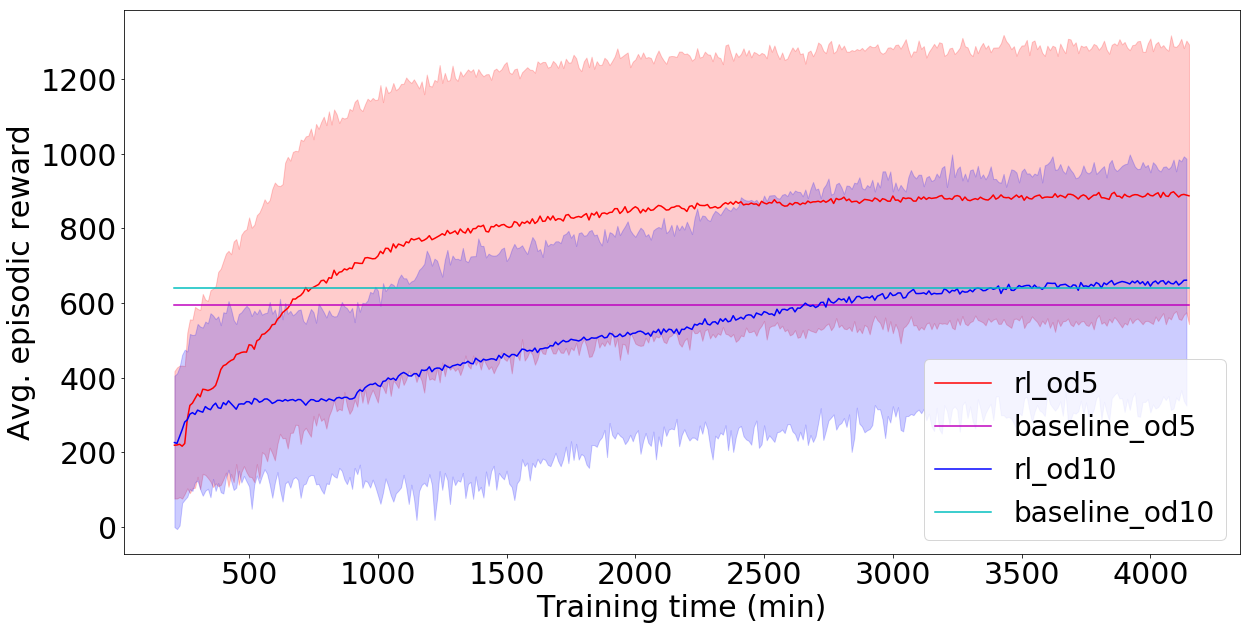
\includegraphics[width=1\linewidth]{vrp_images/vrp_ordernumber.png}
		\caption{RL vs baseline solution for VRP with 2 pick-up locations, map $5 \times 5$, and number of orders 5 and 10. }
		\label{fig:vrp_ordernumber}
	\end{subfigure}
\label{fig:vrp}
\caption{RL vs baseline during policy training process.}
	\vspace{-1em}
\end{figure*}

\subsection{Reinforcement Learning Algorithm}
\label{subsec:vrp_rl}
%We consider a Markov Decision Process (MDP) formulation to tackle this problem and cast the optimal routing path as a sequence of actions that an agent takes. 
\begin{description}[style=unboxed,leftmargin=0cm]
	\item[State:] 
	We include pickup location $\mathbf{p}_t$, driver info $\mathbf{d}_t$, and order info $\mathbf{o}_t$. Driver info contains the driver's position $\mathbf{h}_t$ and the capacity left $c_t$. Order info contains the orders' location $\mathbf{l}_t$, status $\mathbf{w}_t$ (open, accepted, picked up or delivered), the time elapsed since each order's generation $\mathbf{e}_t$ and the corresponding dollar value $\mathbf{v}_t$.  Thus, the state is  $S_t = (\mathbf{p}_t, \mathbf{d}_t, \mathbf{o}_t)$, in which $\mathbf{d}_t = (\mathbf{h}_t, c_t)$, $\mathbf{o}_t = (\mathbf{l}_t, \mathbf{w}_t, \mathbf{e}_t, \mathbf{v}_t)$.
	\item[Action] 
	The agent chooses an action $A_t$ from five options -- accept an order, pick up an accepted order, go to a customer's node for delivery, head to a specific pickup location, or wait and stay unmoved. 
	\item[Reward:] The reward $R_t$ is the total value of all delivered orders $\mathbf{f}_t$ minus the cost $\mathbf{q}$. $\mathbf{f}_t$ is divided into $3$ equal parts for reward shaping: when the order gets accepted, picked up, and delivered respectively. Thus we have:
	\begin{equation*}
			R_t = \frac{1}{3}\Big(\mathbbm{1}_{accepted} + \mathbbm{1}_{picked-up} + \mathbbm{1}_{delievered} \Big) \mathbf{f}_t - \mathbf{q}_t,
	\end{equation*}
	where $\mathbf{q}_t = (q_{time} + q_{move} + q_{failure})$. $q_{time}$ is the time cost, $q_{move}$ is the moving cost (per time step). $q_{failure}$ is a large penalty ($order\_miss\_penalty = 50$) if the agent accepts an order but fails to deliver within the promised time. 
	
\end{description}

The vehicle's capacity remains unchanged if an order is accepted but not picked up. In effect, this grants the agent the flexibility to accept more orders than its capacity, which can be picked up later when space allows. The action of heading to a specific pickup location enables the agent to learn to stay near popular pick up locations. % From a practical perspective, in a case where the majority of the customer orders come from a popular pick-up location, the agent may stay nearby even when there are currently no orders.

%The reward shaping also comes from a practical consideration. In essence, the order value is divided into $3$ parts to encourage order acceptance as well as pick-up, whereas the large penalty $q_{failsure}$ is imposed to prevent the agent from only accepting orders without successful deliveries. This way, we expect the learned policy to be capable of not only making full use of its capacity but also avoiding unsuccessful deliveries. 

We impose action masking during the policy training. The agent cannot perform the following invalid actions: \textit{(i)} pick up an order when its remaining capacity is $0$; \textit{(ii)} pick up an order that is not yet accepted; \textit{(iii)} deliver an order that is not yet picked up. 

To train the policy, we apply the APE-X \cite{horgan2018distributed} DQN algorithm due to its ability to scale by generating more experience replays and picking from them in a distributed prioritized fashion \footnote{We also applied PPO with default hyperparameters provided in RLLib. The reward increased much slower than that of APEX-DQN and was not able to beat baseline after 1-day training.}. We feed the input into a two-layer neural network with 512 hidden units each to compute the Q values. Appendix \ref{appendix:vrp_hp} lists the hyperparameters we use.

\subsection{Results}
For multiple problem scales determined by map size ($map\_size \in \{5 \times 5, 8 \times 8\}$), maximum number of orders ($order \in \{5, 10\}$) and number of pick-up location ($n \in \{2, 3\}$), we conduct experiments to compare the behavior of RL and the MIP baseline solutions. All experiments are conducted in Amazon EC2, where we use \texttt{p3.2xlarge} instances (1 GPU, 16 GPU memory, 8 vCPUs, 61  GB memory and up tp 10 Gbps link). We examine the trained RL policy's ability to generalize to different order distributions. The hyperparameters used for algorithm training are taken from RLLib examples without fine-tuning (Table \ref{table:vrp_hyperparam}). Overall, the RL approach outperforms the baseline across different instance sizes, and generalizes well for unseen order patterns. 

Figure \ref{fig:vrp_mapsize}-\ref{fig:vrp_ordernumber} compares the episodic rewards for the RL policy and the baseline algorithm during training. The shaded band around the mean line shows the minimum and maximum rewards. For readability, the graphs are clipped to skip the initial $3.5$ hours of training as the rewards are highly negative and skew the Y-axis scale. With larger map size or higher order number, the training time required for the agent to achieve rewards equivalent to baseline is higher. This is expected as both the observation and action space increase, the agent requires more exploration to converge to a reasonable policy. Even after three days of training, the rewards for larger instances keep growing gradually. The agent slowly learns to fully utilize the vehicle capacity. Over time, the agent also learns to reject (not accept) orders which are likely to incur penalty. %With more training the RL agent has potential to achieve even higher rewards.

As the agent is trained longer, there is potential for the policy to overfit. In order to test this issue, we train another policy with a shifted hot order-zone distribution ($(0.1, 0.5, 0.3, 0.1)$), and evaluate against the baseline results both using the original order-zone distribution ($(0.5, 0.3, 0.1, 0.1)$). Table \ref{table:vrp_baseline_comp} summarizes the evaluation results. It is observed that the policy is able to outperform the baseline consistently during evaluation phase.
 %The reward during training is lower than that of the baseline, indicating the change we made results in a more difficult senario. However, the policy is able to outperform the baseline consistently during evaluation phase. %In future, we would like to test the agent robustness further by varying the per order rewards and number of zones in the map. 

We also present the rewards with and without the order miss penalty $q_{failure}$ to further understand the agent's behavior about order delivery misses. The reward values are close for problems with less number of pick up locations and fewer orders. As the number of pick-up locations become larger, the gap between the rewards increases. One explanation is the agent cannot multiplex order deliveries from different pick-up locations and the likelihood of missing the order delivery increases. This behavior is also seen if the number of orders is higher. Even though the RL agent reward is better than the baseline, there is still scope for improvement by reducing the number of order delivery misses.

\begin{table}[h!]
	\resizebox{\columnwidth}{!}{%
		\begin{tabular}{|c|cc|c|}
			\hline
			\multicolumn{1}{|l|}{\multirow{2}{*}{Problem Instance}}                          & \multicolumn{2}{|c|}{RL Evaluation Reward}                                                                               & \multirow{2}{*}{MIP Reward} \\
			\multicolumn{1}{|l|}{}                                                                               & \multicolumn{1}{l}{Without $q_{failure}$ }                                 & \multicolumn{1}{l|}{With $q_{failure}$ }                             &                             \\ \hline
			\begin{tabular}[c]{@{}c}5 by 5 map, 5 orders\\ 2 pick-up locations \end{tabular}                    & \begin{tabular}[c]{@{}c@{}}854.45 \\ (136.03)\end{tabular} & \begin{tabular}[c]{@{}c@{}}838.30 \\ (154.12)\end{tabular} & 595.91                      \\ \hline
			\begin{tabular}[c]{@{}c}5 by 5 map, 5 orders\\ 3 pick-up locations\end{tabular}  & \begin{tabular}[c]{@{}c@{}}754.27 \\ (116.48)\end{tabular} & \begin{tabular}[c]{@{}c@{}}730.40 \\ (132.75)\end{tabular} & 642.62                      \\ \hline
			\begin{tabular}[c]{@{}c}5 by 5 map, 10 orders\\ 2 pick-up locations \end{tabular}               & \begin{tabular}[c]{@{}c@{}}774.63 \\ (143.34)\end{tabular} & \begin{tabular}[c]{@{}c@{}}692.34\\ (200.65)\end{tabular}  & 640.01                      \\ \hline
			\begin{tabular}[c]{@{}c}8 by 8 map, 5 orders\\ 2 pick-up locations\end{tabular}                      & \begin{tabular}[c]{@{}c@{}}548.53 \\ (107.40)\end{tabular} & \begin{tabular}[c]{@{}c@{}}536.55 \\ (112.33)\end{tabular} & 410.58                      \\ \hline
			\begin{tabular}[c]{@{}c}8 by 8 map, 5 orders\\ 3 pick-up locations \end{tabular}                          & \begin{tabular}[c]{@{}c@{}}429.20 \\ (102.37)\end{tabular} & \begin{tabular}[c]{@{}c@{}}373.7 \\ (129.98)\end{tabular}  & 246.25                      \\ \hline
		\end{tabular}
	}
	\caption{RL and baseline solution comparison for VRP. Values in the brackets are standard deviations and mean reward is calculated using 50 episodes.}
	\label{table:vrp_baseline_comp}
		\vspace{-1em}
\end{table}

%\begin{table}[h!]
%	\resizebox{\columnwidth}{!}{%
%	\begin{tabular}{|c|c|cc|c|}
%		\hline
%		\multicolumn{1}{|l|}{\multirow{2}{*}{Problem Instance}}                              & \multirow{2}{*}{RL Training Reward} & \multicolumn{2}{c|}{RL Evaluation Reward}                                                                               & \multirow{2}{*}{MIP Reward} \\
%		\multicolumn{1}{|l|}{}                                                               &                                     & \multicolumn{1}{l}{Without $q_{failure}$ }                                 & \multicolumn{1}{l|}{With $q_{failure}$ }                             &                             \\ \hline
%		\begin{tabular}[c]{@{}c@{}}5 by 5 map\\ 2 pick-up locations\\ 5 orders\end{tabular}  & 620                                 & \begin{tabular}[c]{@{}c@{}}854.45 \\ (136.03)\end{tabular} & \begin{tabular}[c]{@{}c@{}}838.30 \\ (154.12)\end{tabular} & 595.91                      \\ \hline
%		\begin{tabular}[c]{@{}c@{}}5 by 5 map\\ 3 pick-up locations\\ 5 orders\end{tabular}  & 570                                 & \begin{tabular}[c]{@{}c@{}}754.27 \\ (116.48)\end{tabular} & \begin{tabular}[c]{@{}c@{}}730.40 \\ (132.75)\end{tabular} & 642.62                      \\ \hline
%		\begin{tabular}[c]{@{}c@{}}5 by 5 map\\ 2 pick-up locations\\ 10 orders\end{tabular} & 592                                 & \begin{tabular}[c]{@{}c@{}}774.63 \\ (143.34)\end{tabular} & \begin{tabular}[c]{@{}c@{}}692.34\\ (200.65)\end{tabular}  & 640.01                      \\ \hline
%		\begin{tabular}[c]{@{}c@{}}8 by 8 map\\ 2 pick-up locations\\ 5 orders\end{tabular}  & 380                                 & \begin{tabular}[c]{@{}c@{}}548.53 \\ (107.40)\end{tabular} & \begin{tabular}[c]{@{}c@{}}536.55 \\ (112.33)\end{tabular} & 410.58                      \\ \hline
%		\begin{tabular}[c]{@{}c@{}}8 by 8 map\\ 3 pick-up locations\\ 5 orders\end{tabular}  & 295                                 & \begin{tabular}[c]{@{}c@{}}429.20 \\ (102.37)\end{tabular} & \begin{tabular}[c]{@{}c@{}}373.7 \\ (129.98)\end{tabular}  & 246.25                      \\ \hline
%	\end{tabular}
%}
%\caption{RL and baseline solution comparison for VRP. Values in the brackets are standard deviations and mean reward is calculated using 50 episodes.}
%\label{table:vrp_baseline_comp}
%\end{table}

%An important observation is that the size of the action and state space of the problem directly impacts the RL agents training. Currently for each additional order the action space grows by three. Having a very large action space makes the policy convergence slow. In future, we want to explore action and space embedding approaches to restrict the action and space space. This would help extent the algorithm to larger problems and still achieve comparable or better rewards. Another important lever in training is reward shaping. In the current formulation we reward the agent with 1/3rd rewards each time it $accepted$, $picked-up$ and $delivered$ order. If the agent fails to deliver we penalize it with late penalty and also take back the partial rewards. Adjusting the reward distribution can help accelerate training and finding optimal policies. Also, training on a larger cluster of machine for more duration can result in much better policies.


%\begin{table}[h!]
%	\resizebox{1\columnwidth}{!}{%
%\begin{tabular}{|c|c|}
%	\hline
%	DQN config                           & Apex config                          \\ \hline
%	\multicolumn{1}{|c|}{dueling: False} & \multicolumn{1}{|c|}{num\_workers: 7} \\
%	double\_q: False                     & num\_gpus: 1                         \\
%	beta\_annealing\_fraction: 1         & sample\_batch\_size: 20              \\
%	prioritized\_replay\_alpha: 0.5      &                                      \\
%	prioritized\_replay\_eps: 0.01       &                                      \\
%	lr: 1e-3                             &                                      \\
%	adam\_epsilon: 1.5e-4                &                                      \\
%	buffer\_size: 1e6                    &                                      \\
%	exploration\_final\_eps: 1e-2        &                                      \\
%	n\_step: 3                           &                                      \\
%	fcnet\_hiddens: {[}512, 512{]}       &                                      \\ \hline
%\end{tabular}
%}
%\caption{Hyperparameters used in the VRP problem. DQN and Apex argument names are consistent with that in \url{https://github.com/ray-project/ray/tree/master/python/ray/rllib}.}
%\label{table:vrp_hyperparam}
%\end{table}



